\documentclass[sigplan,screen]{acmart}
\settopmatter{printfolios=true,printccs=false,printacmref=false} %% max submission space

%% Conference information
\acmConference[REBLS'18]{International Workshop on Reactive and Event-Based Languages & Systems}{November 04--09, 2018}{Boston, MA, USA}
\acmYear{2018}
\acmISBN{}
\acmDOI{}
\startPage{1}
%% Copyright
\setcopyright{none}

%% Recommended packages
\usepackage{booktabs}   % formal tables
\usepackage{subcaption} % complex figures with subfigures/subcaptions
% Math
\usepackage{amsfonts}
% Tikz
\usepackage{tikz}
\usepackage{smartdiagram}
\usetikzlibrary{arrows,mindmap,trees,fit,backgrounds,decorations.pathreplacing,calc,positioning}
\usepackage{environ}
\makeatletter
\newsavebox{\measure@tikzpicture}
\NewEnviron{scaletikzpicturetowidth}[1]{%
  \def\tikz@width{#1}%
  \def\tikzscale{1}\begin{lrbox}{\measure@tikzpicture}%
  \BODY
  \end{lrbox}%
  \pgfmathparse{#1/\wd\measure@tikzpicture}%
  \edef\tikzscale{\pgfmathresult}%
  \BODY
}
\makeatother
% Colors
\usepackage{xcolor}
\colorlet{myrd}{ACMRed}
\colorlet{mygr}{ACMGreen}
\colorlet{mybl}{ACMLightBlue}
\colorlet{mybr}{ACMOrange}
\colorlet{myye}{ACMYellow}
% Images
\graphicspath{ {images/} }
% Code
\usepackage{minted}
% Extra
\usepackage{enumitem}
\usepackage{tabularx}
\usepackage{adjustbox}
\usepackage{url}

\renewcommand{\comment}[1]{}

\begin{document}%\sloppy
% Dataflow graphs
\tikzset{
	dataflow/.style={draw, fill=myye!80, rounded corners, thick},
	empty/.style={draw=none, inner sep=.3cm},
  	machine/.style={draw, fill=myrd!80, rounded corners, thick, inner sep=.3cm},
  	task/.style={draw, fill=mygr!80, rounded corners, thick, inner sep=.5cm},
  	to/.style={->,>=stealth',shorten >=1pt,semithick},
  	net/.style={to, red, dotted},  	
  	opt/.style={->,>=stealth',shorten >=1pt,semithick,draw=red},
  	point/.style={draw, inner sep=0pt, circle, fill=black},
  	every matrix/.style={ampersand replacement=\&, column sep=.7cm, row sep=.35cm},
  	every node/.style={align=center, anchor=base}
}

% General macros
\newcommand\site[1]{\footnote{\url{#1}}}

\newcommand\xdown{%
   \mathrel{\rotatebox{-90}{$\rightsquigarrow{\rule{.03cm}{0pt}}$}}
}

\newcommand\xright{%
   \mathrel{\rotatebox{0}{$\rightsquigarrow{\rule[-2cm]{0pt}{0cm}}$}}
}

\newcommand\myimage[3]{
	\begin{figure}[h!] 
		\centering
	 	\includegraphics[scale=#2]{#1}
	  	\caption{#3}
	  	\label{fig:#1}
	\end{figure}
}

\newcommand\codefig[3]{
	\begin{figure}[h!]
	  \begin{center} \input{diagrams/#1.tikz} \end{center}
		#2
		\caption{#3}
		\label{fig:#1}
	\end{figure}
}

\newcommand\mydiag[2]{
	\begin{figure}[h!] 
		\centering
	 	\input{diagrams/#1.tikz}
	  	\caption{#2}
	  	\label{fig:#1}
	\end{figure}
}

\newcommand\twofig[3]{
	\begin{figure}[h!]
		\begin{center} \input{diagrams/#1.tikz} \end{center}
		$\xdown$
		\begin{center} \input{diagrams/#2.tikz} \end{center}
		\caption{#3}
		\label{fig:#1}
	\end{figure}
}

\newcommand\optimization[3]{
	\begin{figure}[h!]
	  \input{diagrams/optimization/#2B.tikz}
	  \hspace{-.4cm}
	  \input{diagrams/optimization/rightarrow#1.tikz}
	  \hspace{-.4cm}
	  \input{diagrams/optimization/#2A.tikz}
		\caption{#3}
		\label{fig:#2}
	\end{figure}	
}

% Source Code
\usemintedstyle{friendly}
\newcommand\mintedfs{0.2cm}
\newmintedfile[hs]{hs}{frame=lines, framesep=\mintedfs}
\newmintedfile[hssm]{hs}{fontsize=\footnotesize, frame=lines, framesep=\mintedfs}
\newmintedfile[jv]{java}{frame=lines, framesep=\mintedfs}
\newmintedfile[scala]{scala}{frame=lines, framesep=\mintedfs}
\newmintedfile[scalas]{scala}{fontsize=\footnotesize, frame=lines, framesep=\mintedfs}
\newmintedfile[scalaxs]{scala}{fontsize=\tiny, frame=lines, framesep=\mintedfs}
\newmintedfile[jvs]{java}{fontsize=\footnotesize, frame=lines, framesep=\mintedfs}
\newmintedfile[jvxs]{java}{fontsize=\tiny, frame=lines, framesep=\mintedfs}

\title[RHEA]{RHEA: A Reactive, Heterogeneous, Extensible and Abstract Framework for Dataflow Programming}
%\subtitle{}

%% Orestis
\author{Orestis Melkonian}
\orcid{0000-0003-2182-2698}
\affiliation{
  \department{Information and Computing Sciences}
  \institution{Utrecht University}
  \city{Utrecht}
  \country{The Netherlands}
}
\email{o.melkonian@uu.nl}

%% Angelos
\author{Angelos Charalambidis}
\orcid{0000-0001-7437-410X}
\affiliation{
  \department{Institute of Informatics and Telecommunications}
  \institution{NCSR ``Demokritos''}
  \city{Athens}
  \country{Greece}
}
\email{acharal@iit.demokritos.gr}

\begin{abstract}
Robotics and IoT applications are perfect candidates that can benefit from
the functional reactive programming paradigm. Moreover since the typical
program can be represented as a dataflow graph the application can be conceptually
separated and distributed in different machines and the several graph partitions
can run in parallel and possibly in different execution stacks. In this paper
we propose a general-purpose reactive framework that can express complex
applications seamlessly and transparently integrating different sources and
middlewares. The framework is abstract and extensible making it easy to integrate
well-established technologies that rely on the PubSub model. We demonstrate
the usability of the framework by providing applications in the domain of
robotics and IoT.
\end{abstract}

%% 2012 ACM Computing Classification System (CSS) concepts
%% Generate at 'http://dl.acm.org/ccs/ccs.cfm'.
\begin{CCSXML} <ccs2012> <concept>
<concept_id>10011007.10010940.10010971.10010972.10010545</concept_id>
<concept_desc>Software and its engineering~Data flow
architectures</concept_desc> <concept_significance>500</concept_significance>
</concept> <concept>
<concept_id>10011007.10011006.10011008.10011009.10011016</concept_id>
<concept_desc>Software and its engineering~Data flow languages</concept_desc>
<concept_significance>500</concept_significance> </concept> </ccs2012>
\end{CCSXML}

\ccsdesc[500]{Software and its engineering~Data flow architectures}
\ccsdesc[500]{Software and its engineering~Data flow languages}
%% End of generated code


%% Keywords
\keywords{dataflow programming,
          stream processing,
          functional reactive programming (FRP),
          declarative languages,
          implicit concurrency,
          node placement}

\maketitle

\section{Introduction} \label{sec:introduction}

A typical application in Robotics or Internet of Things (IoT) needs to timely and
continuously respond to time-varying external sensory data and as a result the
reactivity of these applications is imperative. Typically, the programmer of such
applications has to deal with asynchronous callbacks in conventional imperative
programming languages in order to implement tedious and often error-prone behaviours
that should comply with the reactive requirements.

%\paragraph{Why FRP is popular and many systems embrace it}
A promising and relatively recent proposal for simplifying the implementation of
reactive applications is the \emph{functional reactive programming} (FRP) \cite{fran}.
FRP makes heavy use of higher-order functional operators to define, essentially, a
dataflow network of processing nodes. These high-level abstractions
alleviates, as intended, the low-level implementation chores. FRP was originally proposed
though as a framework for developing graphical user interfaces but fortunately the key
high-level abstractions are generic enough that other domains can benefit from this
approach. As a result of its generality and its popularity several general-purpose
implementations emerge with different capabilities and prerequisites.

It is natural, therefore, to investigate whether robotics and IoT applications
can fit into this new paradigm. Indeed most robotic applications follow the
Robot Perception Architecture, where inputs to system are the robot's
sensors, which are then processed by a dataflow graph, whose output is given as
commands to the robot actuators. Moreover, robotics typically involve several
different other robotic or IoT systems to enhance their sensing abilities. This
combination naturally give rise to issues of distributing the dataflow graph to
several robotic units and issues of heterogeneity and interoperability between
different middlewares and protocols.

The first steps towards using FRP in robotics was identified in \cite{arrows_robots}
and realized in Yampa\site{https://wiki.haskell.org/Yampa}, an FRP framework
developed in Haskell. Yampa provides its functionality through an embedded DSL
as it is customary for many of the FRP libraries. Although an interesting proposal,
there is limited acceptance from the robotics community mainly because it does
not integrate well with existing well-established robotics middlewares such as
the Robot Operating System (ROS)~\cite{ROS}. Moreover, it does assume distributed execution
and integration with other systems via the Reactive Streams Standard\site{http://www.reactive-streams.org}.

Motivated by the robotics and IoT community we propose \textsc{RHEA}, an abstract
FRP general-purpose framework that aims to act as a unifying layer that can
be mapped and executed simultaneously using different reactive libraries
and existing middlewares such as ROS and MQTT. The programmer can transparently
express a complex reactive applications within this framework that may use
both sensing from several robots and IoT sensors. The framework places the
dataflow nodes to computational resources and handles the serialization needed
between different execution engines.

%\paragraph{Structure of the paper}
The rest of the paper is structured as follows.
Section~\ref{sec:background} provides some background context about dataflows and
the state-of-art middlewares used in robotics and IoT.
Section~\ref{sec:requirements} discusses the main requirements and objectives that drove the design of the framework.
Section~\ref{sec:approach} presents the framework's characteristics and capabilities.
Section~\ref{sec:implementation} discusses implementation details and
Section~\ref{sec:distributed} presents the techniques used for distributed execution.
Section~\ref{sec:optimization} presents several optimizations that have been implemented in the
framework. Section~\ref{sec:applications} demonstrates some use-cases of the framework
mainly motivated by robotics and IoT.
Section~\ref{sec:related} discusses related work and
finally Section~\ref{sec:conclusions} concludes with future directions.

\section{Background} \label{sec:background}
In this section we provide some background context needed. In particular, we
briefly present the dataflow model and the notation of graphs we use in the
remaining paper. We continue with a brief overview of the well-established
middlewares used in robotics and IoT, namely the Robot Operating System (ROS)
and the Message Queuing Telemetry Trasport (MQTT) protocol.
Moreover, for the rest of the paper we assume familiarity with the functional
reactive programming (FRP).

\subsection{The Dataflow Computational Model}
In the dataflow computational model, the program is represented as a dataflow graph, where
nodes are independent computational units and edges are communication channels
between these units. A node is fired immediately when its required inputs are
available and therefore no explicit control commands are needed for execution.
An immediate consequence is that the nodes of the graph can run independently
and potentially in parallel as soon as their inputs are present.

%\begin{example}
Figure~\ref{fig:nat} shows a dataflow graph enumerating the set $\mathbb{N}$ of
natural numbers.
%
\mydiag{nat}{Natural numbers}
%
In the dataflow graph above, we can discern three types of nodes: sources, which
do not have any incoming edge and act as value generators to initiate
computation, sinks, which do not have any outgoing edges and inner nodes, which
transform one or more incoming streams and redirect their output to other nodes.
The \textit{zero} node just produces a stream with a single value 0 and then
terminates. \textit{Concat} produces a single stream by concatenating the stream
produced by \textit{zero} and \textit{increment}, while \textit{increment}
transforms its input stream by adding one to its values. Finally, the sink node
displays the result, which is the stream of natural numbers.

Streams can be infinite, such as the stream produced by \textit{concat} because
it is the concatenation of a single-value stream and an infinite one. Moreover,
the graph is cyclic as \textit{concat} feeds input to \textit{increment} and
vice versa. The most interesting fact is that there nodes are independent and
therefore can run in parallel. For instance, while \textit{increment} is
processing value 5 (i.e. to produce value 6), the previous result (i.e. value 5)
passes through \textit{concat} to reach the sink node, which can concurrently
process it to display it.
%\end{example}

Dataflow graphs can be executed both in a single-machine and in cluster of
machines where each node can be placed in a different machine. A possible
single-machine implementation could represent edges as in-memory queues,
whereas a multi-machine one could realize them as channels between TCP sockets,
allowing communication across the network.

\comment{%
\subsection{Functional reactive programming}

A relatively recent programming paradigm is \textit{Functional Reactive
Programming (FRP)}, which provides a conceptual framework for implementing
reactive (i.e. time-varying and responding to external stimuli) behaviour in
\textit{hybrid systems} (i.e. containing both continuous and discrete
components), such as robots, in functional programming languages.

\textit{FRP} first appeared as a composable library for graphic animations
~\cite{fran}, but quickly evolved into a generic paradigm
~\cite{survey_frp,pushpull_frp}. Moreover, extensive research has
investigated \textit{FRP} as a framework for robotics
~\cite{arrows_robots,lambda_in_motion}.

Although appealing at first, \textit{FRP} was not appropriate for systems  with
real-time constraints, due to uncontrollable time- and space- leaks
~\cite{event_frp}. The solution was a generalization of monads called
\textit{arrows}~\cite{arrows}, which provided the necessary guarantees that the
aforementioned common errors do not occur.

The main advantages of \textit{FRP} are its close correspondence to
mathematics~\cite{survey_frp}, which make it an ideal framework for modelling
real-time systems, and its concise representation of time-varying values via
\textit{signals}.

\paragraph{The Reactive Streams Standard}
The \textit{Reactive Streams Standard (RSS)} is an initiative
to provide a standard for asynchronous stream processing with non-blocking back
pressure. This encompasses efforts aimed at runtime environments (JVM and
JavaScript) as well as network protocols~\cite{rss}.

\textit{RSS} defines two minimal interfaces for the roles of \textit{Subscriber}
and \textit{Publisher}~\cite{rss_docs}.
A \textit{Subscriber} implementation should define
reactions to observed values, including normal and erroneous termination,
whereas a \textit{Publisher} implementation should accept requests from
\textit{Subscribers} and start emitting values to them.
}

\subsection{Robotics and IoT Middlewares}
In the following we briefly present the ROS and MQTT, the de-facto middlewares
used in robotics and IoT. The architecture of both follow a topic-based
publish-subscribe (PubSub) pattern to loosely couple different processes and
at the same time maximize flexibility.

\subsubsection{ROS}
\textit{ROS} is an open-source middleware for robot software, which emphasizes
large-scale integrative robotics research~\cite{ROS}. It provides a \textit{thin}
communication layer between heterogeneous computers, from robots to mainframes
and it has been widely adopted by the research community around the world, due
to its flexibility and maximal support of reusability through packaging and
composability. It provides a compact solution to the development complexity
introduced by complex robot applications that consist of several modules and
require different device drivers for each individual robot.

It follows a peer-to-peer network topology, implemented using a topic-based
\textit{PubSub} messaging protocol and its architecture reflects many sound
design principles. Another great property of \textit{ROS} is that it is
language-agnostic, meaning that only a minimal specification language for
message transaction has been defined, so contributors are free to implement
small-size clients in different programming languages, with \textit{roscpp} for C++
and \textit{rospy} for Python being the most widely used ones.

A typical development scenario is to write several \textit{nodes}, that
subscribe to some topics and, after doing some computation, publish their
results on other topics. The main architectural issue here is that subscribing
is realized through asynchronous callback functions, so complicated schemes
easily lead to unstructured code, which obviously lead to unreadable and
hard-to-maintain code. Our approach gives a solution to the aforementioned
problem.

\subsubsection{MQTT}
Internet of Things (IoT) conveys the concept of a multitude of heterogeneous devices,
ranging from low-cost sensors to vehicles with embedded electronics, are connected and
provide the ability to collect data and exchange it amongst themselves.
The development of such systems though, due to their heterogeneity, is rather
complex and costly. Recent development of a variety of middleware frameworks,
showed that a standard protocol of communication is imperative along with supporting
tools~\cite{iot_middleware}.

The most widely spread protocol is \textit{MQTT}, which follows the \textit{PubSub}
messaging pattern and provides a very minimal and lightweight communication layer
in order not to put a strain on the resource-bounded system~\cite{mqtt}.
For instance, an \textit{IoT} application could connect to some sensors by
subscribing to their corresponding topics, taking decisions that would result in
some commands to some actuators, by publishing to their corresponding topics.

Fortunately, the dataflow model seems to be rather fitting for these
scenarios~\cite{iot_dataflow}, as every node in the graph is completely
independent, and consequently can be any "\textit{thing}". This useful property
of the model makes it a good architectural choice for such applications. The
only thing to consider is how these things will communicate in a standard way,
so as to be able to add new types of \textit{things} and integrate it in an
effortless way to an existing dataflow network.

\section{The RHEA Framework} \label{sec:approach}

\subsection{Requirements and Objectives} \label{sec:requirements}

%\paragraph{Reactive}
The system should be \textit{reactive}, as close as possible to the definition
of the Reactive Manifesto\site{http://www.reactivemanifesto.org}. In particular,
the system should be
\begin{description}
  \item[responsive] meaning it should be able to handle successfully time-sensitive scenarios if at all possible.
  This is the cornerstone of usability and utility.
  \item[resilient] meaning it is able to recover robustly and gracefully after
  a failure, due to the fact that nodes in the dataflow graph are completely
  independent and recovery of each one can be done in isolation.

%Another thing to note here is that special error messages are built-in and make
%it very easy to propagate errors between \textit{components}, in case the error-
%handling part of a component is decoupled from the computational logic. This
%leads to much more robust architectures for large-scale systems, where fault-
%tolerance is mission-critical.

  \item[elastic] meaning it will adjust itself depending on the available resources
  and demanded workload. For instance, the granularity of the graph (i.e. number of nodes)
  is adjusted so as to match a heuristic-based value (e.g. total number of threads).

  \item[message-driven] meaning it relies solely on asynchronous message-passing
  for inter-component communication leading to loose coupling, isolation, location
  transparency and the error propagation.
\end{description}

%\paragraph{Heterogeneous}
One of the major concerns while designing the framework was the ability to
deploy it anywhere, from low-cost robots to mainframes. Apparently such
attribute would require a very flexible runtime environment that have the ability to handle
\textit{heterogeneous} devices.

%\paragraph{Extensible}
As the new technologies and frameworks arise the system should be able to adapt
and be extended in order to remain useful and general-purpose.
Therefore, careful consideration was taken to compose the system of different
independent modules, which could \textit{extensible} and easily modified. With that concept
in mind, generality and abstraction were heavily emphasized during both the design
and the implementation process.

%\paragraph{Abstract}
The framework should be also \textit{abstract} in terms of implementation details,
as it is completely agnostic of any machine-specific requirements. It is designed as a
unifying conceptual base for further extensions and careful consideration was
taken not to restrict in any aspect.

\subsection{Architecture}
The \textsc{RHEA} framework consists of several clearly separated modules,
whose interconnection is illustrated in Figure~\ref{fig:architecture}.
%
\begin{figure*}
  \centering
  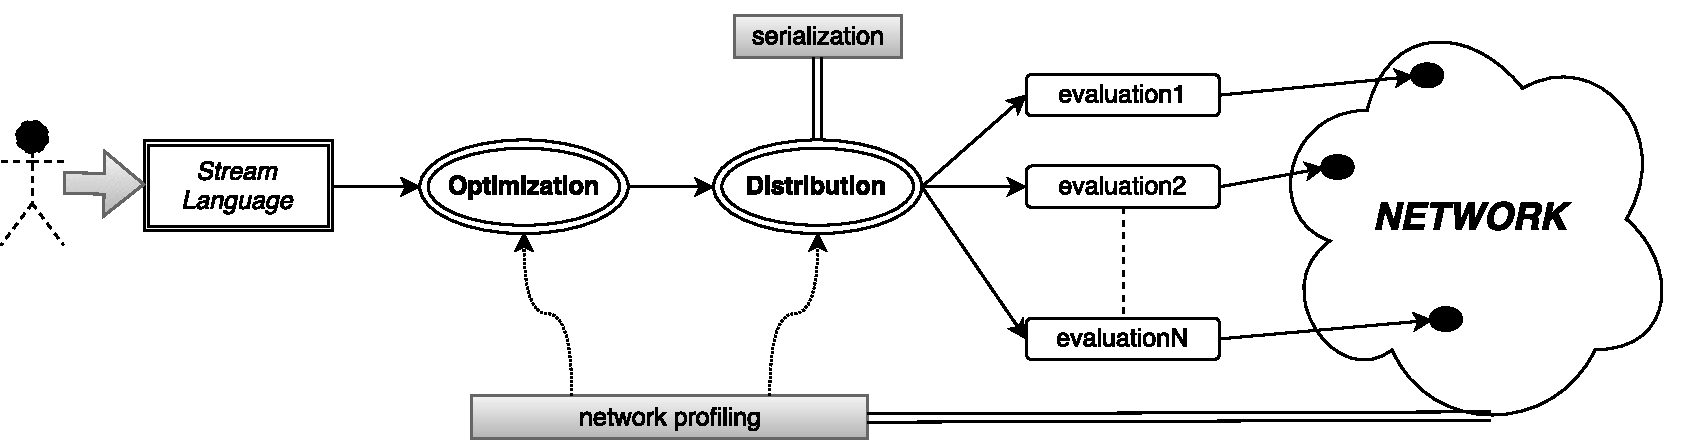
\includegraphics[scale=0.6]{architecture}
    \caption{System architecture}
    \label{fig:architecture}
\end{figure*}

A typical workflow of the system has as follows. The user writes a program in
the provided domain-specific language, which constructs an internal representation
of the dataflow graph. Afterwards, using information about the available
resources in the network, the constructed graph is optimized and partitions of the
graph are assigned to physical computational resources. The optimized graph partitions are
then distributed across the available machines for execution, maybe using a
different evaluation strategy each time.

More specifically, a flexible evaluation strategy was employed where different
executors can be considered when available. This design satisfies the requirements
of extensibility, heterogeneity and abstraction of the system since each partial
graph can be evaluated by a different \textit{EvaluationStrategy} which could
interpret it using a specific streams library or even compile into CUDA code
for execution on a GPU. In Section~\ref{sec:implementation} we provide three
different evaluation strategies.

\subsection{Dataflow Graphs}

The kind of dataflow graph that can be expressed using the framework's stream
language are directed cyclic graphs with possibly many inputs and outputs.
%
%\paragraph{The Stream data type}
The data channels (i.e. edges of the dataflow graph) are represented using the
\texttt{Stream} data type, which is parametric, meaning that it can emit values
of any data type, whether built-in or user-defined. The stream produced may
terminate, successfully or erroneously, or even be infinite.

%\paragraph{Graph construction syntax}
The construction of the internal dataflow graph is implicit, through a
rich set of operators on the Stream data type. Each \texttt{Stream} object
contains internally a dataflow graph of type \texttt{FlowGraph}, which is only
to be accessed and manipulated by the internal module, evaluation strategies and
optimizers. Therefore, an application developer only needs to work with the
\texttt{Stream} type.

Source nodes are constructed using built-in functions of type \texttt{Stream}.
For instance, \texttt{Stream.just(1, 2, 3)} produces the stream that emits just
the values 1, 2 and 3. The return variable of these creation function is an
object of type \texttt{Stream}.

Processing nodes can be divided into two classes: \textit{single input} ones and
\textit{multiple input} ones.
%
Single input nodes are inserted into an existing \texttt{Stream} object, by
calling an operator on that object.
Multiple input nodes are constructed by built-in function that take as
argument already existing \texttt{Stream} objects.

\codefigg{singleinput}{\jvs{code/singleinput.java}}{Single input processing node}
%
\codefigg{multipleinput}{\jvs{code/multipleinput.java}}{Multiple input processing node}
%
Figure~\ref{fig:singleinput} shows an
example of a single input node, namely that of \texttt{map}, which transforms
the input stream (i.e. just the values 1, 2 and 3) by applying a user-defined
function to every emitted value.
%
Figure~\ref{fig:multipleinput} shows
an example of a multiple input node, namely that of \texttt{zip}, which
transforms the input streams by
applying a user-defined function to each emitted pairs of values.
Here we also see the stream creation function \texttt{Stream.range}.
%

The variables returned by all processing nodes are \texttt{Stream} objects. These
objects can be reused in different parts of the graph to enable splitting a
node's output to different processing nodes or outputs. Figure~\ref{fig:split}
shows such an example, where the \texttt{filter} operator only emits values for
which the given function returns true.

Cycles are constructed using the \texttt{loop} operator, which is a single
input processing node. It requires a function that, given an input stream,
constructs a subgraph that redirects its output to that input, therefore
creating a feedback loop. Figure~\ref{fig:natt} shows an example of the
\texttt{loop} operator to represent the natural numbers, just as the graph
shown earlier in Figure~\ref{fig:nat}. The \texttt{concat} operator is a
multiple input node that concatenates its input streams.

\codefigg{split}{\jvs{code/split.java}}{Split example}
\codefigg{natt}{\jvs{code/natt.java}}{Cyclic example}

%\paragraph{Evaluation syntax and semantics}
Lastly, to evaluate a given dataflow graph and do something with its output values, we
need to call the \texttt{subscribe} method of the \texttt{Stream} object and pass as argument
a user-defined action (i.e. function with side-effects).
%
%The execution is completely asynchronous, hence the order of stream
%declaration and evaluation does not matter at all.

\section{Implementation} \label{sec:implementation}

Since extensibility is a major design priority, most individual critical
components are defined using the Strategy design pattern, isolating the desired
functionality in a separate interface and allowing the system to select the
appropriate instantiating classes at runtime. The main pluggable components of
the system, for which default implementations are already provided by the
current implementation as separate libraries, are \textit{Evaluation},
\textit{Optimization}, \textit{Distribution}, \textit{Serialization} and
\textit{Network Profiling}.

%\paragraph{Notifications}
Every value passed through the framework's streams is wrapped inside a
\texttt{Notification} object, which discriminates stream values into three
categories: \texttt{onNext} (when the stream provides a regular value),
\texttt{onError} (when an error occurs) and \texttt{onComplete} (when the
stream completes its output). This enables the system to handle gracefully
error propagation.

In order to make the framework easy to integrate with other stream and
dataflow technologies, every input and output node implements the interfaces
that RSS defines, namely the Publisher and the Subscriber interface. This also
enables users to define new types of sources or sinks, in order to integrate
the framework with other general technologies (e.g. system events, HTTP requests,
PubSub implementations, etc).
%
In particular, a sink node (output) should implement the Subscriber interface, which
essentially defines three methods corresponding to reactions to a
\texttt{Notification}, one for each of the categories mentioned above.
%
Moreover, a source node (input) should implement the Publisher interface, which defines a
single method \texttt{subscribe(Subscriber)}, where a Subscriber requests the
Publisher to start emitting values.

Many existing technologies provide these interfaces, or at least adapters from
their internal representations, and therefore they are very easy to be
integrated to the framework.

\subsection{Execution}

Every primitive operator corresponds to an expression implementing the
\texttt{Transformer} interface and a complete dataflow is defined by a
\texttt{Stream} variable and an object implementing the \texttt{Output} interface,
which can be either an \texttt{Action}, a \texttt{Sink} or a list of these.

Roughly speaking, the \texttt{EvaluationStrategy} interface accepts the
\texttt{Stream} variable and its corresponding \texttt{Output} and executes it,
however desired. The strategies we have implemented so far follow:
\begin{description}
\item[RxJavaEvaluationStrategy]
which uses RxJava~\site{http://github.com/ReactiveX/RxJava}, an established and well-maintained library for
asynchronous programming using the \textit{Observable} type, which is very close,
semantically, to our \textit{Stream} type.

\item[RosEvaluationStrategy] which integrates the \textit{ROS} middleware into the
framework. This strategy's main objective is to set up a \textit{ROS} client and
configure every \texttt{RosTopic} used within the dataflow that needs to be
evaluated to use this client. After that, evaluation is propagated to a generic
strategy, for example, to RxJavaEvaluationStrategy.

\item[MqttEvaluationStrategy] which integrates the MQTT middleware into the
framework, in the same way \textit{ROS} is integrated.

\end{description}

\subsection{Distributed Execution} \label{sec:distributed}

An evaluation strategy executes the requested dataflow graph in a single
machine, without concern about distribution and resource utilization.
%
For distribution and cluster management, one needs to implement
the \texttt{DistributionStrategy} interface by adjusting the granularity (i.e. size) of
the graph to evaluate to fit the available resources (see, Section~\ref{sec:optimization})
and partition it across all computational resources, maybe using different evaluation strategies.

%\paragraph{Hazelcast}
The default \texttt{DistributionStrategy} uses the \textit{Hazelcast}\footnote{\url{http://hazelcast.org/}}
library to discover and manage multiple machines and used its internal decentralized PubSub model
to communicate intermediate results across the network. Figure~\ref{fig:partition}
illustrates the partitioning of a dataflow graph over several machines, where each
machine -- except the last one -- outputs its result to a Hazelcast topic,
from which another machine gets its input.
%
\optimizationL{2}{partition}{Partitioning}

%\paragraph{Machine configuration}
According to the distribution strategy being used, the available machines will
require a certain initial configuration. For the Hazelcast case, a
little piece of setup code needs to be executed on every member of the cluster,
which is together with the main \texttt{EvaluationStrategy} class. Moreover, helpful
information can also be added at this step, such as number of CPU cores. It is
the distribution strategy's responsibility to ensure that this information is
properly distributed and handled.

Apart from this initial configuration, the distribution strategy needs to enable
members to declare certain capabilities that they possess, which are required by
specialized nodes. For instance, a source node emitting values from a ROS topic
must be executed on a machine having ROS installed, in order to set up a ROS
client. The default implementation uses strings to represent capabilities and
are declared in the initialization code of each machine separately.

\subsubsection{Serialization}
As communication between machines across a network is mandatory, data types
emitted through the streams must be serialized on departure and de-serialized on
arrival at each machine. For this reason, each \texttt{DistributionStrategy}
must be configured with a class implementing the \texttt{Serializer} interface,
but we also provide a default one that covers most datatypes.
Figure~\ref{fig:serialization} depicts the serialization process in more detail.

\mydiag{serialization}{Serialization process}

\section{Optimizations} \label{sec:optimization}

This section describes three stages of optimization the dataflow graph goes
through before being evaluated, which are illustrated in Figure~\ref{fig:optimization}.
The purpose of the optimization graph is to achieve better performance and
utilization of the available resources.

\mydiag{optimization}{Optimization stages}

\subsection{Proactive filtering}

The first optimization stage is a heuristic one, based on the fact that if a
filter operation can be moved earlier (i.e. closer to source nodes) while
preserving the original semantics, then there will be benefit concerning
computational cost and cross-machine communication overhead. The figures below
illustrate one representative example of each general class of
graph transformation.

\optimization{1}{maptake}{Take/skip/distinct before map}
\optimization{1}{mapfilter}{Filter before map}
\optimization{3}{concatdistinct}{Filter/distinct before concat/merge}

\subsection{Granularity adjustment}

Different nodes of the dataflow graph will be executed on a separate
thread/process. The fact that graphs can grow very big, for instance when
programming a swarm of robots, poses a problem when available
computational resources are limited. For this reason, the second optimization
stage tries to adjust the granularity of the dataflow graph to a desired value,
which is normally the number of available threads amongst all machines.

To reach the desired granularity, the optimizer applies some semantic-preserving
transformation, as shown in the figures below.

\optimization{1}{mergemap}{Merge maps}
\optimization{1}{combmapfilter}{Combine map with filter}
\optimization{1}{combfilterexists}{Combine filter with exists}
\optimization{1}{combmapexists}{Combine map with exists}
\optimization{2}{combmapzip}{Combine map with zip}
\optimization{1}{combzipmap}{Combine zip with map}

In Figure~\ref{fig:mergemap} we merge two \textit{map} operations into
one \textit{map} operation that uses the composition of the two initial
functions, while in Figure~\ref{fig:combmapfilter} a \textit{map} followed
by a \textit{filter} is substituted by a more complex equivalent operation,
namely \textit{filterMap}. In figures \ref{fig:combfilterexists} and
\ref{fig:combmapexists} we apply some simple properties of the boolean functions
involved to decrease the number of nodes. Lastly, in figures \ref{fig:combmapzip} and
\ref{fig:combzipmap} we utilize function composition to embed \textit{map}
operations into \textit{zip} operations.

\subsection{Node placement}

After the first two passes, we have an optimized dataflow graph with fine-tuned
granularity. At this stage, nodes are mapped to tasks and are deployed across
the available machines, keeping resource utilization in mind.

If the desired granularity has not been reached yet, the
\textit{DistributionStrategy} applies fusion to pairs of tasks until it reaches
it, as shown in Figure~\ref{fig:fusion}.

\optimization{1}{fusion}{Task fusion}

The final decision to be made is where each of these newly constructed tasks
will be executed, although some of them need to necessarily be placed on
specific machines with certain skills.

Apart from these hard constraints, we need to minimize communication overhead.
For this purpose, one must implement the \textit{NetworkProfileStrategy} by providing
a way to calculate network distance between available machines, which is then fed as input
to the \textit{NodePlacement} optimizer.

\section{Applications} \label{sec:applications}

\subsection{Hamming numbers}

Consider the problem of enumerating the
\textit{Hamming numbers}, which are generated by the mathematical formula
$\mathbb{H} = 2^i3^j5^k$, where $i,j,k \in \mathbb{N}$. There is an intuitive
dataflow solution to the above problem, taken from the book of \textit{Lucid},
which is the first functional dataflow language~\cite{lucid}. Figure
\ref{fig:hamming} shows the dataflow graph with its corresponding \textsc{RHEA}
code.

\codefig{hamming}{\scalaxs{code/hamming.scala}}{Hamming numbers}

The code is written in Scala to utilize the \textit{Pimp my library} design
pattern~\cite{pimp}, which is used to easily add new functions to already
existing libraries, using Scala's \textit{implicit conversions} (line 28). In
the example above, we define two new Stream operators, namely \textit{multiply}
(line 10), which just multiplies the stream with a constant, and
\textit{mergeSort} (line 13), which produces an ordered stream given two ordered
streams as input. We also see the power of the \textit{loop} operator (line 2),
which allows us to define cycles in an effortless manner.

\subsection{Robot control panel}

This application concerns real-time monitoring of a robot, that is publishing
its information and sensor-data to \textit{ROS} topics, through a
\textit{graphical user interface (GUI)}.

The \textit{/camera/rgb} topic provides the frames of the robot's camera as
coloured images, while the \textit{/camera/depth} provides frames that provide
depth information. The \textit{/tf} topic publishes parent-child relations of
the internal topics of the robot's configuration, and finally the
\textit{/scan/} topic provides information from the robot's laser that gives
horizontal depth information in polar coordinates.

The GUI displays the laser data embedded on the camera stream, while allowing
for real-time face detection. Additionally, it displays the depth frames and the
\textit{tf} relations as a tree. Finally, a mock-up battery bar is displayed to
show-case the framework's ability for simulation. Figure~\ref{fig:control_panel}
illustrates the dataflow solution to the above problem and its corresponding
\textsc{RHEA} code.

\codefig{control_panel}{\jvxs{code/control_panel.java}}{Robot control panel}

The implementation details (i.e. the visualization class and methods
\textit{faceDetect}(line 7), \textit{embedLaser}(line 8) and
\textit{toGray}(line 26)) are not shown for brevity's sake. It is evident that
this model of programming encourages a clean separation of concerns between the
individual components, namely between the sensor data manipulation and the
actual visualization on the GUI.

\subsection{Robot hospital guide}

As a final example, we will examine a more IoT-based application. Consider a
robot that guides patients to different parts of a hospital, such as the gym or
cafeteria. Assuming map localization, path finding and obstacle avoidance are
already implemented, there still remains a problem with calibrating the robot's
speed according to the patient's status.

To keep tract of the patient's distance from the robot, each patient carries a
smart-phone that acts as a \textit{bluetooth low-energy (BLE) beacon}. The robot
uses its bluetooth receiver to publish the distance from the signal source to an
\textit{MQTT} topic, which is then transformed by our stream application to
velocity commands for the robot, in the form of slowing down or speeding up.

The first module constitutes the main program logic, where a declared dataflow
graph acts as a stream transformation from beacon information to velocity
commands to the robot. Figure~\ref{fig:hospital} shows the dataflow graph with
its corresponding \textsc{RHEA} code.

\codefig{hospital}{\jvxs{code/hospital.java}}{Robot hospital guide}

The second module just uses the library \textit{ReactiveBeacons}\footnote{\url{http://github.com/ 1083 pwittchen/ReactiveBeacons}}
to get a stream of beacon data via \textit{rxjava}, and then publishes it to a \textit{MQTT} topic,
which is the input of the first module. The corresponding \textsc{RHEA} code
follows:
\jvxs{code/rxbeacon.java}

This example clearly show-cases the framework's ability to combine different
technologies and act as a high-level, declarative coordination language.

\section{Related Work} \label{sec:related}

\subsection{Dataflow systems}

The necessity for implicit parallelism and distribution of more and more
applications, dealing with huge and/or complex data, has brought increasingly
more attention to the dataflow programming model. The main reason many
frameworks have adopted it, is the high level of abstraction it provides with
its declarative approach, making it simple to structure and maintain a complex
system, while at the same time not losing its expressive power.

%\paragraph{Spark}
A very well-known and well-adapted framework for scalable large-data processing
is Apache's \textit{Spark}~\cite{spark}. Although not a
dataflow framework, it was developed to overcome the shortcomings of the
\textit{MapReduce}, similar to \textit{FlumeJava}, by providing a much more
efficient and flexible runtime, offering a rich set of data-parallel operators ($\simeq 80$)
that can be used interactively from Scala, Python, Java or R.

It follows the same general approach as \textsc{RHEA}, in the sense that it is
completely generic and encourages domain-specific libraries to be built upon it.
For instance, \textit{MLib} is a library for machine learning and
\textit{GraphX} is a library for iterative graph algorithms, both stacked upon
\textit{Spark}.

%\paragraph{Akka}
Definitely one the most mature frameworks for distribution targeting the JVM,
\textit{Akka}~\site{http://akka.io} is a toolkit and runtime for highly
concurrent, distributed and resilient message-driven applications.
Its approach follows the \textit{Actor} model, where one perceives
abstract computational agents, called actors, that are distributed in space and
communicate with point-to-point messages that are buffered in a queue. In
reaction to a message, an actor can create more actors, make local decisions,
send more messages and determine how to respond to the next message received.

Similar to the problem of \textit{ROS} that our framework solved, which is the
inappropriate nature of callbacks for complex scenarios, \textit{Akka}
developers also felt the necessity for a more flexible and composable
programming model, so they developed the \textit{AkkaStreams} library, which
provides a convenient API for stream processing and also dataflow graph
construction with an interesting DSL.

The main reason \textsc{RHEA} offers a more flexible solution to \textit{ROS}
shortcomings than \textit{Akka}, is that \textit{Akka} is a pretty heavyweight
library, and consequently may prove over-abundant for simple use-cases. On the
other hand, \textsc{RHEA} offers the ability to choose between several
\textit{EvaluationStrategies} to match your application's needs, therefore a
simple application would just use a lightweight library like \textit{rxjava}.

\subsection{Unified dataflow languages}
%\paragraph{Cloud Dataflow}
Continuing the search for more expressive models, Google recently released the
\textit{Cloud Dataflow} framework~\site{http://cloud.google.com/dataflow/},
which is an evolution of \textit{FlumeJava}~\cite{flumejava}, allowing cycles and
therefore incremental computation.
It is a completely domain-agnostic dataflow framework integrated with many other
closely-related technologies from Google, like Cloud Storage, Cloud PubSub,
Cloud Datastore, Cloud Bigtable and BigQuery.
It is open-source, offers fully automatic resource management that auto-scales
for optimal throughput and provides increased reliability and data consistency.
Moreover, it provides a unified programming model through its API, while
allowing data monitoring and demand-driven execution.

In contrast to \textsc{RHEA}, graphs constructed by \textit{Cloud Dataflow} are
designed to be deployed only on cloud infrastructures, and therefore no support
for complete heterogeneity is provided. In terms of network optimization, namely
node placement,  \textit{Cloud Dataflow} lets the cloud system targeted to make
all decisions, while \textsc{RHEA} profiles the network and decides
autonomously.

%\paragraph{dispel4py}
A less-known framework for Python is
\textit{dispel4py}~\cite{dispel4py}. It provides the ability
to describe abstract workflows for distributed data-intensive applications.
Similar to our \textit{EvaluationStrategy} concept, it allows different mappings
to enactment systems, such as MPI and Apache Storm.
Its main disadvantages are that it has only an API for Python and only allows
low-level specification of the graph's nodes, through the definition of
\textit{Processing Elements}. Therefore, it is inconvenient to compose larger
graphs from simpler ones and the source code becomes chaotic and difficult to
maintain.

\subsection{Dataflow optimization}
%\paragraph{Stratosphere}
The frameworks discussed so far follow, more or less, an imperative approach,
which enables automatic distribution and concurrency by using immutable data
structures. \textit{Stratosphere}~\cite{stratosphere}, on the other hand, follows
a declarative programming approach similar to \textsc{RHEA}, which enables
writing highly parallel code directly from the language's semantics.

Apart from offering a language of a much higher abstraction level,
\textit{Stratosphere} has internalised several interesting and novel approaches
to optimization of dataflow graphs, especially concerning cyclic graphs (i.e.
incremental computation)~\cite{spinning}. These optimizations are generic, in the
sense that most frameworks can adopt them without much effort. Integrating these
optimization into \textsc{RHEA}, as future work, would certainly be of great
benefit to the performance of the system.

\subsection{Heterogeneous data processing}
Another dataflow framework from Google is
\textit{TensorFlow}~\cite{tensorflow}, which is an open-source
polyglot library for machine learning and especially construction of neural
networks.
The interesting fact is that, although it started out as a rigid neural network
library, it quickly generalized to a dataflow construction library, much similar
to our own project, which started out as a robotics library.
Its main features are its portability to multiple computational architetures
(e.g. CPU, GPU) and multiple language APIs (e.g. C++, Python), although
its main advantage are its domain-specific operators for neural nets (i.e.
common subgraphs, auto-differentiation).
Through the edges/streams connecting the nodes, only a single but flexible data
type is allowed, namely the \textit{Tensor} type, which essentially is a multi-
dimensional array that usually represents features or weights. In contrast to
\textsc{RHEA}'s Streams, \textit{Tensors} cannot be infinite, mainly due to the
fact that their size is determined by the dimensionality of the problem being
solved, which is, in most cases, a fixed constant.


\subsection{Robotics and IoT}

It is only natural that the dataflow model would make its way through the field
of robotics, as many behaviours in control theory are expressed as dataflow
diagrams.

%\paragraph{roshask}
\textit{Roshask}~\cite{roshask} is a binding from the Haskell programming language
to the basic \textit{ROS} interfaces. Like \textsc{RHEA}, the approach is to
overcome the shortcomings of \textit{ROS} callbacks by viewing topics as
streams. This allows for, and encourages, a higher level of abstraction in
robot programming, while making the fusing, transforming and filtering of
streams fully generic and compositional.
%\paragraph{Yampa}
\textsc{RHEA} and \textit{roshask} were heavily influenced by the work of Hudak's
group (Yale Haskell Group) on robot DSLs and FRP in general~\cite{fran,arrows_robots,lambda_in_motion}.
\textit{Yampa}~\cite{arrows_robots} is a DSL embedded in Haskell
that realizes the FRP model, using arrows to minimize time-/space- leaks.

%\subsection{Internet of Things}

IoT applications often deal with much heterogeneity, due to the variety of
sources that different devices introduce. Therefore, a component-based approach
suits well to solve this problem and there are some dataflow frameworks that
follow that approach.
%\paragraph{Node-RED}
Another interesting \textit{IoT} tool for JavaScript following a dataflow
approach is \textit{Node-RED}~\cite{iot_dataflow}, which is a visual tool for wiring
together hardware devices, APIs and online services in new and interesting ways.
Applications called flows, are built immediately on a browser, and can be
deployed on the Cloud with just a single click. The main advantage of this tool
is that it encourages social development, due to the fact that flows are stored
in JSON format, which can be easily imported and exported for sharing with
others.

\section{Conclusions and Future Work} \label{sec:conclusions}

The framework described in this paper was designed with extensibility in mind,
aiming to act as a fundamental basis, onto which various domain-specific
libraries or DSLs will rely in the future. To that end, a constant effort to
generalize and make components as abstract as possible was made.

The set of operators aided expressibility, making it possible to specify any
dataflow graph in a concise and readable manner. This disallowed optimizations
suitable for less expressive models (e.g. \textit{Map-Reduce}), but recent
research has shown that general dataflow topologies have optimization
opportunities that are yet to be found~\cite{blackbox}. A minimal optimization
stage has been implemented, which paves the path to more advanced optimization
techniques, such as those used in \textit{Naiad}~\cite{naiad} and
\textit{Stratosphere}~\cite{blackbox}.

The extensible nature of \textsc{RHEA} allows for many meaningful extensions, such as
more evaluation/distribution strategies to support integration with other software ecosystems,
Moreover, the design of a block-based visual language interface would certainly make the
framework even more accessible to novice programmers and smooth the learning curve
associated with dataflow programming.

There are also significant shortcomings to the framework design and implementation that
could be addressed in future work.
For instance, \textit{dynamic reconfiguration} is needed to handle environments that are constantly changing.
A concrete contribution to the \textsc{RHEA} would be to integrate \textit{HotWave}~\cite{reconf_java},
which is an \textit{aspect-oriented programming (AOP)} framework that supports dynamic
(re)weaving of previously loaded classes. This would allow the user to specify the desired
adaptive behaviour for reconfiguring where nodes are executed, what operation they perform, and so forth.

Another major drawback is that network profiling - an integral part of node placement - is achieved via
calculation of \textit{round-trip time (RTT)}, which is naively expensive and may outweigh the benefits of
exploiting network proximity. A possible decentralized approach that we could employ would be the \textit{Vivaldi}
coordinate system~\cite{vivaldi}, which assigns synthetic coordinates to hosts
such that the distance between the coordinates of two hosts accurately predicts
the communication latency between them.

A last major drawback that ultimately needs to be addressed is fault-tolerance,
since there are no advanced methods for specifying behaviour for graceful
error-recovery. This is essential for large machine clusters, in which systems it is
certain that host failures and other faults will be a common occurrence. The
functional nature of the dataflow model enables fault-tolerance, in addition to
parallelism, due to the fact that a node can be moved to another machine for
execution, while preserving the original semantics.  This contribution path can draw
heavy influence from recent research on fault-tolerance for stream processing engines~\cite{borealis},
which provide efficient models for availability and data recovery/consistency,
by using data replication and parallel recovery of lost state.

The applications demonstrated the framework's ability to provide a higher level
of abstraction, where the language only specifies how different components
coordinate, without knowledge of the implementation details. This is exactly
what \textit{Ziria} accomplishes in the domain of wireless systems
programming~\cite{ziria}. The driving force for both frameworks is that some
specific domains have fixated their methods on low-level programming, whereas
more satisfactory paradigms can solve many shortcomings.

%% Bibliography style
\bibliographystyle{ACM-Reference-Format}
%% Citation style
\citestyle{acmnumeric}  % acmauthoryear
%% Bibliography
\bibliography{rhea}

\end{document}
